\subsection{Trực quan hóa: Ánh xạ tĩnh}
PostHistory [438] khai phá trực quan các mẫu hình (pattern) hoạt động e-mail khác nhau (ví dụ: các mạng xã hội, tốc độ trao đổi e-mail) và vai trò của thời gian trong các mô hình này (xem Hình (\ref{fig:f7.12})). PostHistory lấy người dùng làm trung tâm và tập trung vào các tương tác trực tiếp của một người dùng với những người khác thông qua e-mail. Các mẫu hình được tạo ra từ việc phân tích thông tin tiêu đề e-mail. Vì vậy, không phải nội dung của thư, mà lưu lượng được lưu vết mới là yếu tố được sử dụng làm cơ sở để phân tích các e-mail trao đổi của mọi người theo thời gian. Về cơ bản, giao diện người dùng trực quan hóa hoạt động trao đổi e-mail trong cả một năm và giao diện này được chia thành hai bảng chính: bảng lịch ở bên trái và bảng danh bạ ở bên phải. Bảng lịch hiển thị cường độ hoạt động e-mail hàng ngày trong đó mỗi ô vuông biểu thị một ngày và mỗi hàng biểu thị một tuần. Kích thước của hình vuông được xác định bởi số lượng e-mail nhận được vào ngày đó và màu sắc của nó thể hiện hướng trung bình tính của thư (tức là thư được nhận qua hình thức TO, CC hay BCC). Màu sắc càng sáng thể hiện các thư nhận được trong ngày hôm đó càng được định hướng rõ ràng. Bảng danh bạ được sử dụng để hiển thị tên của những người đã gửi e-mail cho người dùng.
\begin{figure}[H] % places figure environment here   
    \centering % Centers Graphic
    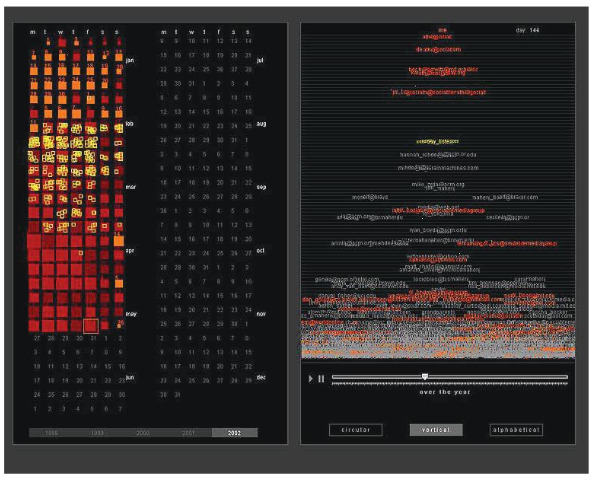
\includegraphics[width=0.8\textwidth]{assets/fig_7_12.png} 
    \caption{PostHistory [438]. Bảng lịch ở bên trái hiển thị hoạt động e-mail hàng ngày, trong đó số lượng e-mail và hướng trung bình của chúng được lần lượt thể hiện bởi kích thước và màu sắc của các hộp vuông tương ứng. Bảng danh bạ ở bên phải hiển thị tên của những người đã gửi e-mail cho người dùng.} % Creates caption underneath graph
    \label{fig:f7.12}
\end{figure}